%Sweave("spatial_inla.Rnw", encoding="UTF-8", keep.source=FALSE)
%system("pdflatex spatial_inla.tex")
%system("bibtex spatial_inla")
\documentclass[article]{jss}

\usepackage{thumbpdf}
\usepackage{amssymb}



%%%%%%%%%%%%%%%%%%%%%%%%%%%%%%
%% declarations for jss.cls %%%%%%%%%%%%%%%%%%%%%%%%%%%%%%%%%%%%%%%%%%
%%%%%%%%%%%%%%%%%%%%%%%%%%%%%%

%% almost as usual
\author{Roger S. Bivand\\NHH Norwegian\\ School of Economics \And 
Virgilio G\'omez-Rubio\\Universidad de\\ Castilla-La Mancha 
\And H\r{a}vard Rue\\Norwegian University for\\ Science and Technology
%Achim Zeileis\\Universit\"at Innsbruck \And 
%        Second Author\\Plus Affiliation}
}
\title{Extending the \pkg{R-INLA} Package for Spatial Statistics}

%% for pretty printing and a nice hypersummary also set:
\Plainauthor{Roger S. Bivand, Virgilio G\'omez-Rubio, H\r{a}vard Rue}
\Plaintitle{Extending the R-INLA Package for Spatial Statistics}
%\Shorttitle{} %% a short title (if necessary)

%% an abstract and keywords
\Abstract{
The Integrated Nested Laplace Approximation (INLA) provides an interesting
way of approximating the posterior marginals of a wide range of Bayesian
hierarchical models. This approximation is based on conducting a 
Laplace Approximation of certain functions and numerical integration is
extensively to integrate some of the models parameters out. 

INLA is implemented in the \pkg{R-INLA} package, which provides a suitable
interface for data analysis. Although the INLA methodology can deal with
a large number of models, only the most relevant have been implemented
within \pkg{R-INLA}. However, many other important models are not available
for \pkg{R-INLA} yet.

In this paper we show how to extend the number of latent models available
for the model parameters. Our approach is based on conditioning on one
or several model parameters and fit these conditioned models with \pkg{R-INLA}.
Then these models are combined using Bayesian Models Averaging to provide
the final approximations to the posterior marginals of the model.

Finally, we show some examples of the application of this technique
in spatial statistics. It is worth noting that our approach can be extended
to a number of other fields, and not only spatial statistics.


}
\Keywords{INLA, spatial statistics, \proglang{R}}
\Plainkeywords{INLA, spatial statistics, R}
%% at least one keyword must be supplied

%% publication information
%% NOTE: Typically, this can be left commented and will be filled out by the technical editor
%% \Volume{50}
%% \Issue{9}
%% \Month{June}
%% \Year{2012}
%% \Submitdate{2012-06-04}
%% \Acceptdate{2012-06-04}

%% The address of (at least) one author should be given
%% in the following format:
\Address{
Roger S. Bivand\\
Department of Economics\\
NHH Norwegian School of Economics\\
Helleveien 30\\
N-5045 Bergen, Norway\\
 \\
%}
%\Address{
Virgilio G\'omez-Rubio\\
Department of Mathematics\\
School of Industrial Engineering\\
University of Castilla-La Mancha\\
02071 Albacete, Spain\\
 \\
%}
%\Address{
H\r{a}vard Rue\\
Department of Mathematical Sciences\\
Norwegian University for Science and Technology\\
N-7491 Trondheim, Norway
}

\usepackage{Sweave}
\begin{document}

\section[Introduction]{Introduction}


Bayesian inference has become very popular in spatial statistics in recent
years. Part of this success is due to the availability of computation methods
to tackle fitting of spatial models. \citet{besagetal:1991} proposed in their
seminal paper an appropriate way of fitting a spatial model using Markov Chain
Monte Carlo methods. This model have been extensively used and extended to
consider different types of fixed and random effects for spatial and
spatio-temporal analysis.

In general, fitting these models have been possible because of the availability
of different computational techniques, being Markov Chain Monte Carlo the most
notable. For large models or big data sets, MCMC can be tedious and reaching
the required number of samples can take a long time. Not to mention that
autocorrelation may arise and that an increased number of iterations may be
required.

Alternatively, the posterior distributions of the parameters could be
approximated in some way. However, most models are highly multivarite and
approximating the full posterior distribution may not be possible in practice.
The Integrated Nested Laplace Approximation \citep[][INLA]{isi:000264374200002} focuses on
the posterior marginals for latent Gaussian models. Although these may seem
a strong constraint, these models appear in a good number of fields. 
Hence, INLA will be particularly useful when  only
marginal inference on the model parameters.

The \pkg{R-INLA} package\citep{rinla:2013} for the \proglang{R} programming language provides
an implementation of INLA so that models can be fitted using standard 
\proglang{R} commands. Results are readily available for plotting or
further analysis. Although INLA is a general method to approximate the
posterior marginals, \pkg{R-INLA} implements a few latent models and prior
distributions for the model parameters.
This may be a drawback, as it is difficult to fit new models with INLA if these
are based on other distributions not available in \pkg{R-INLA}.  This may be an
inconvenience when trying to develop new models as there is no easy way of
extending \pkg{R-INLA} to fit other models.

We have deivsed a way of extending the number of models that \pkg{R-INLA} can
fit with little extra effort. First of all, we consider one (or more)
parameters in our model so that, if they are fixed, the resulting model can be
fitted with \pkg{R-INLA}. What we are doing here is, in fact, fit a model
conditioned on the assigned values to the parameters. Then, we can assign
different values to these parameters and combine the resulting models in some
way to obtain a fit of the original model. We have used Bayesian Model
Averaging and numerical integration techniques to combine these models.


This paper is organised as follows. Section \ref{sec:INLA} describes
the Integrated Nested Laplace Approximation.  In Section \ref{sec:spmodels}
the different latent models for spatial statistics are described.
We describe how to extend \pkg{R-INLA} to fit new models in Section
\ref{sec:extINLA}. Some examples are provided in Section{sec:examples}.
Finally, we discuss why our approach is relevant in Section \ref{sec:disc}.

\section{Integrated Nested Laplace Approximation}
\label{sec:INLA}

Bayesian inference is based on computing the posterior distribution of a
vector of model parameters $\mathbf{x}$ conditioned on the vector of observed
data $\mathbf{y}$. Bayes' rule states that this posterior distribution
can be written down as

$$
\pi(\mathbf{x}|\mathbf{y}) \propto \pi(\mathbf{y}|\mathbf{x}) \pi(\mathbf{x})
$$
\noindent
Here, $\pi(\mathbf{y}|\mathbf{x})$ is the likelihood of the model and
$\pi(\mathbf{x})$ represents the prior distribution on the model parameters.


Usually, $\pi(\mathbf{x}|\mathbf{y})$ is a highly multivariate distribution
and difficult to obtain. In particular, it is seldom possible to derive it in
a closed form. For this reason, several computational approaches  have been 
proposed to get approximations to it. MCMC is probably the most widely used
family of computational approaches to estimates the posterior distribution.

The marginal distributions can be denoted by $\pi(x_i|\mathbf{y})$
and it can be easily derived from the full posterior by integrating
out over the remaining set of parameters $\mathbf{x}_{-i}$.

Let us assume that we have a set of $n$ observations 
$\mathbf{y}=\{y_i\}_ {i=1}^n$, whose distribution is of the Exponential family.
The mean of observation $i$ is $\mu_i$, which is modelled using a linear
predictor $\eta_i$ as follows:

$$
\eta_i=\alpha+\sum_{j=1}^{n_f} f^{(j)}(u_{ji})+\sum_{k=1}^{n_{\beta}}\beta_k z_{ki}+\varepsilon_i
$$
\noindent
$\alpha$ is the intercep, $f^{(j)}$ are functions on a set of $n_f$ random
effects on a vector of covariates $\mathbf{u}$, $\beta_k$ are coefficient on
some covariates $\mathbf{z}$ and $\varepsilon_i$ are error terms. Hence, the
vector of latent effects is $\mathbf{x}=\{\{\eta_i\}, \alpha, \{\beta_k\},
\ldots\}$. Note that given our particular interest in spatial models, terms
$f^{(j)}(u_{ji})$ can be defined as to model spatial or spatio-temporal
dependence.

$\mathbf{x}$ is modelled using a Gaussian distribution with zero mean and
variance-covariance matrix $Q(\theta_1)$. Now, $\theta_1$ is a vector of
hyperparameters. Furthermore, $\mathbf{x}$ is supposed to be a Gaussian Markov
Random Field \citep[GMRF,][]{rueheld:2005}. This means that  $Q(\theta_1)$ will fullfil a number of
Markov properties. 
%This will make $y_i$ independent given $x_i$ and $\theta$.

The distribution of observations $y_i$ will depend on the latent effects
$\mathbf{x}$ and, possibly, a number of hyperparameters $\theta_2$.  Taking
the vector of hyperparameters $\theta=(\theta_1, \theta_2)$, observations
$y_i$ will be independent of each other $x_i$ and $\theta$ because
of $\mathbf{x}$ being a GMRF.

Following \citet{isi:000264374200002}, the posterior distribution of the model
latent effects $\mathbf{x}$ and hyperparameters $\theta$ can be written as 

$$
\pi(\mathbf{x}, \mathbf{\theta}|\mathbf{y}) \propto
\pi(\mathbf{\theta}) \pi(\mathbf{x}|\mathbf{\theta})\prod_{i\in \mathcal{I}}\pi(y_i|x_i,\mathbf{\theta})
\propto 
$$

$$
\pi(\mathbf{\theta}) |\mathbf{Q}(\mathbf{\theta})|^{n/2} \exp\{-\frac{1}{2}\mathbf{x}^T \mathbf{Q}(\mathbf{\theta}) \mathbf{x}+\sum_{i\in\mathcal{I}} \log(\pi(y_i|x_i, \mathbf{\theta}) \}
$$
\noindent
$\mathcal{I}$ represents an index of observed data (from 1 to $n$),
$\mathbf{Q}(\mathbf{\theta})$ is a variance-covariance matrix on some
hyperparameters $\theta$ and $\log(\pi(y_i|x_i, \mathbf{\theta}) \}$ is
the log-likelihood of observation $y_i$.

INLA allows different forms for the likelihood of the observations.  This
includes not only distributions from the Exponential family but also mixtures
of distributions. Also, INLA can handle observations with different likelihoods
in the same model. Regarding the latent effects $\mathbf{x}$, different models
can be used. We will describe some of these in more detail in Section
\ref{sec:spmodels}.


The specification of the prior distributions $\pi(\theta)$ is also very 
flexible. These will often depend on the latent effect but, in principle,
the most common distributions are available and the user can define its
own prior distribution in the \pkg{R-INLA} package (but we will come
back to this later). 

Hence, we can write the marginals distributions of the elements in $\mathbf{x}$
and $\mathbf{\theta}$ (i.e., latent effects and hyper-parameters) as


$$
\pi(x_i|\mathbf{y}) \propto \int \pi(x_i|\mathbf{\theta}, \mathbf{y})  \pi(\mathbf{\theta}| \mathbf{y}) d\mathbf{\theta}
$$
\noindent
and

$$
\pi(\theta_j|\mathbf{y}) \propto \int \pi(\mathbf{\theta}| \mathbf{y})  d\mathbf{\theta}_{-j} 
$$

In order to estimate the previous marginals, we need 
$\pi(\mathbf{\theta}|\mathbf{y})$ or, alternatively, a convenient
approximation that the will denote by $\tilde\pi(\theta|\mathbf{y})$.
Intially, this approximation can be taken as

$$
\tilde\pi(\mathbf{\theta}|\mathbf{y})\propto 
\frac{\pi(\mathbf{x},\mathbf{\theta},\mathbf{y})}{\tilde\pi_G(\mathbf{x}|\mathbf{\theta},\mathbf{y})}\bigg|_{x=x^*(\theta)}
$$
\noindent
Here 
$\tilde\pi_G(\mathbf{x}|\mathbf{\theta},\mathbf{y})$ is a Gaussian
approximation to the full conditional of $\mathbf{x}$ and $x^*(\theta)$
is the mode of the full conditional for a given value of $\mathbf{\theta}$.
\citet{isi:000264374200002} take this approximation and use it 
to compute the marginal distribution of $x_i$ using numerical integration:

$$
\tilde\pi(x_i|\mathbf{y})= 
\sum_k \tilde\pi (x_i|\mathbf{\theta}_k, \mathbf{y})\times 
\tilde\pi(\mathbf{\theta}_k|\mathbf{y})\times \Delta_k
$$
\noindent
Here $\Delta_k$ are the weights associated to vector of values
$\mathbf{\theta}_k$ in a grid for vector of hyperparameters .

%\citet{isi:000264374200002}  also discuss how the approximation $\tilde\pi
%(x_i|\mathbf{\theta}_k, \mathbf{y})$ should be in order to reduce numerical
%error and they provide different alternatives.

Note that in the previous equation it is important to have good approximations
to $\pi (x_i|\mathbf{\theta}_k, \mathbf{y})$. A Gaussian approximation
$\tilde\pi_G (x_i|\mathbf{\theta}_k, \mathbf{y})$, with mean $\mu_i(\theta)$
and variance $\sigma^2_i(\theta)$, may be a good starting point but a better
approximation may be required in other cases. \citet{isi:000264374200002}
developed better approximations based on alternative approximation methods,
such as the Laplace Approximation.  For example, they have used the Laplace
Approximation to obtain:

$$
\tilde\pi_{LA}(x_i|\mathbf{\theta}, \mathbf{y}) \propto 
\frac{\pi(\mathbf{x}, \mathbf{\theta}, \mathbf{y})}
{\tilde\pi_{GG}(\mathbf{x}_{-i}|x_i, \mathbf{\theta}, \mathbf{y})}
\bigg|_{\mathbf{x}_{-i}=\mathbf{x}^*_{-i}(x_i, \mathbf{\theta})}
$$
\noindent
$\tilde\pi_{GG}(\mathbf{x}_{-i}|x_i, \mathbf{\theta}, \mathbf{y})$ is a
Gaussian  approximation to $\mathbf{x}_{-i}|x_i, \mathbf{\theta}, \mathbf{y}$
around its mode $\mathbf{x}^*_{-i}(x_i, \mathbf{\theta})$.

\citet{isi:000264374200002} develop a Simplified Laplace Approximation to
improve $\tilde\pi_{LA}(x_i|\mathbf{\theta}, \mathbf{y})$ using a series
expansion of the Laplace Approximation around $x_i$. This approximation is
computationally less expensive, and it also corrects for location and
skewness.


\subsection[The R-INLA package]{The \pkg{R-INLA} package}

INLA has been implemented as an \proglang{R} package called \pkg{R-INLA},
which can be downloaded from \url{http://www.r-inla.org/}. \pkg{R-INLA}
provides an interface similar to the one used to fit Generalized Additive
Models with function \code{gam()}. It can handle fixed effects, non-linear terms
and random effects in a \code{formula} argument. The interface is flexible
enough to allow for the specification of different priors and model fitting
options. Non-linear terms and random effects are included in the formula as
calls to the \code{f()} function. 


The model is fitted with a call to function \code{inla()}, which will return an
\code{inla} object with the fitted model. Note that, by default, only a number
of results will be returned. These includes the marginal distributions of
the latent effects and hyperparameters. 


In addition to the posterior marginals, \pkg{R-INLA} can provide a number
of additional quantities on the fitted model. For example, it can 
provide the log-marginal likelihood $\pi(\mathbf{y})$ which can be used
for model selection. Other model selection criteria such as the DIC 
\citep{Spiegelhalteretal:2002} and CPO \citep{Heldetal:2010}.

Furthermore, \pkg{R-INLA} includes a number of options to define the
prior distributions for the parameters in the model. Well-known
prior distributions are available and the user can define his own prior
distributions as well.

In the next Section we describe different examples of the use of
\pkg{R-INLA} for spatial statistics. Therein we have included
a detailed description on how \code{inla()} should be called.

\section{Spatial models with INLA} \label{sec:spmodels}


As discussed in Section \ref{sec:INLA}, spatial dependence can be included as
part of the vector of latent effects $\mathbf{x}$. In principle, any number of
random effects can be included in the model. In this Section, we will describe
the different options available, depending on the type of problem. A full
description of the models described here can be found in the \pkg{R-INLA}
website at \url{http://www.r-inla.org}, but we have included here a summary
here. \citet{Blangiardoetal:2013} and \citet{GomezRubioetal:2013} also discuss
the different spatial models included in \pkg{R-INLA}.

\subsection{Analysis of lattice data}

First of all, we will discuss the analysis of lattice data because this will
set the basis for other types of analyses. In the analysis of lattice data
observations are grouped according to a set of areas, which usually represent
some sort of administrative region (neighbourhoods, municipalities, provincies,
countries, etc.).

\pkg{R-INLA} includes a latent model for uncorrelated random effects. In
this case, the random effects $u_i$ are modelled as

\begin{equation}
u_i \sim N(0, \tau_u)
\end{equation}
\noindent
where $\tau_u$ refers to the precision of the Gaussian distribution.  It should
be noted that \pkg{R-INLA} assigns a prior to $\log(\tau_u)$ which, by default,
it is a Gaussian distribution with zero mean and fixed precision.  Although
this model is not spatial, it can be combined with other spatial models.


In order to model spatial correlation, neighbourhood must be set among the
study areas.  It is often considered that two areas are neighbours is they
share a common boundary.  Spatial autocorrelation is modeled using a Gaussian
distribution with zero mean and a precision matrix that will model
correlation between neighbours. Given that latent effects are GMRF, 
we can define the variance-covariance matrix of the random effects
as

$$
\Sigma = \frac{1}{\tau} Q^{-1}
$$
\noindent
where $\tau$ is a common variance parameter and matrix $Q$ encodes
the spatial structure. Given that we are assuming a latent GMRF, this also
means that matrix $Q$ will be defined such as element $Q_{ij}$ is zero if
areas $i$ and $j$ are not neighbours. This means that $Q$ is often a very
sparse matrix. See, for example, \citet{rueheld:2005} 
for details.

Available specifications for spatial dependence includes the intrinsic CAR
specification \citep{besagetal:1991}. This will produce a $Q$ matrix in which
element $Q_{ii}$ is $n_i$ (the number of neighbours of area $i$) and element
$Q_{ij},\neq j$ is -1 if areas $i$ and $j$ are neighbours and 0 otherwise. This
means that the spatial random effects $v_i$ are distributed as

$$
v_i|v_j,\tau_v N( \frac{1}{n_i}\sum_{i\sim j} v_j, \frac{1}{\tau_vn_i})\ i\neq j
$$
\noindent
$\tau_v$ is the conditional precision of the random effects. As in the previous
model, \pkg{R-INLA} uses a Gaussian prior on $\log(\tau_v)$.

In addition, a proper version of this model is available as well,
for which the spatial random effects are distributed as

$$
v_i|v_j,\tau_v N( \frac{1}{n_i+d}\sum_{i\sim j} v_j, \frac{1}{\tau_v(n_i+d)})\ i\neq j
$$
\noindent
$d$ is a positive quantity to make the distribution proper. By default,
a log-Gamma distribution is assigned to $\log(d)$.

A more general approach is obtained  with the following precision
matrix:

$$
Q = (I - \frac{\rho}{\lambda_{max}}C)
$$
\noindent
Here $I$ is the identity matrix, $\rho$ a spatial autocorrelation parameter,
$C$ an adjacency matrix and $\lambda_{max}$ the maximum eigenvalue of $C$.
This specification ensures that $\rho$ takes values between 0 and 1.
\pkg{R-INLA} assigns a Gaussian prior on $\log(\rho/(1-\rho))$.

In the following example we use the \code{boston} data set from the
\proglang{R} package \pkg{spdep} to develop an example on several spatial
models.  This data set  records median price for houses that were occupied by
their owners plus some other relevant covariates \citep[see,][for
details]{HarrisonRubinfeld:1978}. Data have been recorded at the tract level
and the neighbourhood structure of the tracts is also available.
We have converted this into a binary matrix to be used with \pkg{R-INLA}
using function \code{nd2mat}. This will be passed to function \code{f()} when
defining the spatial model.

A summary of some latent models implemented in \pkg{R-INLA}, and that can be
used within the \code{f()} function, is available in Table
\ref{tab:inlamodels}. Note that this is not an exhaustive list and that a
complete list of the available latent models can be obtanined from the
\pkg{R-INLA} documentation. Also, detailed examples are available from the
\pkg{R-INLA} website at \url{http://www.r-inla.org}.


\begin{table}[h]
\begin{center}
\begin{tabular}{ll}
Name in \code{f()}  & Model \\
\hline
\code{besag} & Intrinsic CAR\\
\code{besagproper} & Proper CAR\\ 
\code{bym} & Convolution model \\
\code{rw2d} & 2-D random walk \\
%\hline[.25cm]
\code{generic0} & $\Sigma=\frac{1}{\tau}Q^{-1}$ \\[.25cm]
\code{generic1} & $\Sigma=\frac{1}{\tau}(I_n-\frac{\rho}{\lambda_max}C)^{-1}$
%\code{rw2d} & Random walk of order 2
\end{tabular}
\end{center}
\caption{Summary of some latent models implemented in \pkg{R-INLA} 
for spatial statistics.}
\label{tab:inlamodels}
\end{table}



The model that we are fitting is:

$$
y_i = \alpha+\beta X + u_i +\varepsilon_i
$$
\noindent
where $\alpha$ is the model intercept, $\beta$ a vector of coefficients
of the covariates, $v_i$ a random effect with an intrinsic CAR specification
and $\varepsilon_i$ is random Gaussian error term.



\begin{Schunk}
\begin{Sinput}
> library("spdep")
> library("maptools")
> data("boston")
> library("INLA")
> adj<- nb2mat(boston.soi, style="B")
> boston.c$ID<-1:nrow(boston.c)
> form<-log(CMEDV) ~ CRIM + ZN + INDUS + CHAS + I(NOX^2) + I(RM^2) +  AGE + 
+ log(DIS) + log(RAD) + TAX + PTRATIO + B + log(LSTAT)+
+ f(ID, model="besag", graph=adj )
> m1<-inla(form, data=boston.c)
\end{Sinput}
\end{Schunk}

Note how the call to \code{inla()} is similar to fitting other regression
models with \proglang{R} with \code{glm()} or \code{gam()}. Furthermore, 
it is very easy to include spatial random effects with function \code{f()}
in the \code{formula} passed to \code{inla()}.


A summary of the model can be obtained as
follows:

\begin{Schunk}
\begin{Sinput}
> summary(m1)
\end{Sinput}
\begin{Soutput}
Call:
"inla(formula = form, data = boston.c)"

Time used:
 Pre-processing    Running inla Post-processing           Total 
          0.711           1.651           0.135           2.497 

Fixed effects:
               mean     sd 0.025quant 0.5quant 0.975quant kld
(Intercept)  3.5323 0.1595     3.2192   3.5325     3.8449   0
CRIM        -0.0051 0.0009    -0.0069  -0.0051    -0.0033   0
ZN           0.0004 0.0005    -0.0005   0.0004     0.0013   0
INDUS       -0.0004 0.0025    -0.0052  -0.0004     0.0045   0
CHAS1       -0.0285 0.0273    -0.0821  -0.0285     0.0251   0
I(NOX^2)    -0.1136 0.1506    -0.4088  -0.1137     0.1822   0
I(RM^2)      0.0108 0.0011     0.0087   0.0108     0.0128   0
AGE         -0.0013 0.0005    -0.0022  -0.0013    -0.0004   0
log(DIS)    -0.0938 0.0689    -0.2291  -0.0939     0.0415   0
log(RAD)     0.0513 0.0200     0.0120   0.0513     0.0905   0
TAX         -0.0004 0.0001    -0.0006  -0.0004    -0.0002   0
PTRATIO     -0.0169 0.0051    -0.0269  -0.0169    -0.0070   0
B            0.0007 0.0001     0.0005   0.0007     0.0009   0
log(LSTAT)  -0.2295 0.0216    -0.2719  -0.2295    -0.1870   0

Random effects:
Name	  Model
 ID   Besags ICAR model 

Model hyperparameters:
                                        mean    sd      0.025quant 0.5quant
Precision for the Gaussian observations 408.385 176.137 197.624    365.026 
Precision for ID                         23.499   2.956  17.629     23.576 
                                        0.975quant
Precision for the Gaussian observations 863.394   
Precision for ID                         29.115   

Expected number of effective parameters(std dev): 388.82(38.53)
Number of equivalent replicates : 1.301 

Marginal Likelihood:  -108.27 
CPO and PIT are computed
\end{Soutput}
\end{Schunk}
\noindent
The summary includes summary statistics of the posterior marginals of the
coefficients of the fixed effects plus the precisions of the instrinsic CAR
random effect and the error term. Figure \ref{fig:marg1} shows the estimated
marginals of the precisions in the model.

\begin{figure}[h]
\begin{center}
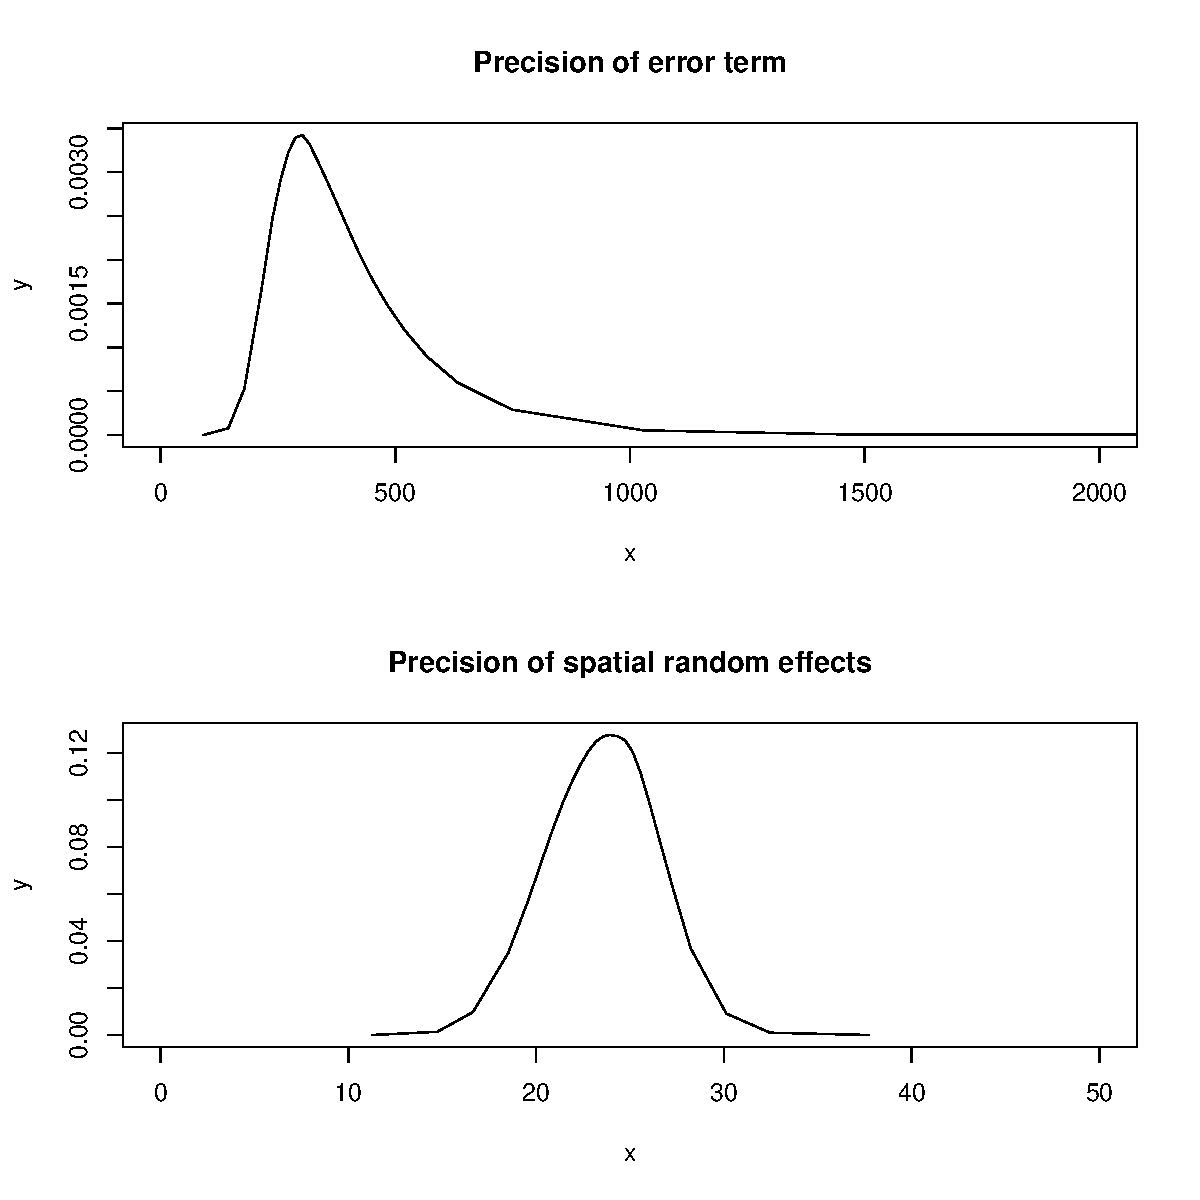
\includegraphics{spatial_inla-004}
\end{center}
\caption{Marginals of the precisions of the error term (top) and
spatial random effects (bottom), Boston housing data.}
\label{fig:marg1}
\end{figure}


\subsection{Point patterns}

Point patterns are analysed with INLA as the result of a counting process,
i.e., points are not modelled directly but they are aggregated over a a grid
of small squares. For this reason, the analysis of point patterns is conducted
similarly to that of lattice data: counts are available for each square and 
these are assigned neighbours according to the adjacent squares. Then, counts
can be smoothed using an appropriate non-linear term, such as spatial
random effects.

In the following example we use the Japanese black pine data set from
\proglang{R} package \pkg{spatstat}. This data set records the location of
Japanese black pine saplings in a square sampling in a natural forest.  This
is example is reproduced from \citet{GomezRubioetal:2013}.

Hence, we first split the study are into smaller squares to create a
grid, and the we aggregate the pines over the grid of squares. 

\begin{Schunk}
\begin{Sinput}
> library("spatstat")
> data("japanesepines")
> japd <- as.data.frame(japanesepines)
> nrow <- 10
> ncol <- 10
> n <- nrow * ncol
> grd <- GridTopology(cellcentre.offset = c(0, 0), cellsize = c(1/9, 
+     1/9), cells.dim = c(nrow, ncol))
> polygrdjap <- as(grd, "SpatialPolygons")
> idxpp <- overlay(SpatialPoints(japd), polygrdjap)
> japgrd <- SpatialGridDataFrame(grd, data.frame(Ntrees = rep(0, 
+     n)))
> tidxpp <- table(idxpp)
> japgrd$Ntrees[as.numeric(names(tidxpp))] <- tidxpp
\end{Sinput}
\end{Schunk}


Next, an index variable is built to create the spatial neighbourhood structure
to be passed to the \code{f()} function. Note that care must be taken as
\proglang{R} and \pkg{R-INLA} may have a different ordering of the areas when
defining the adjacency matrix.

\begin{Schunk}
\begin{Sinput}
> japgrd$SPIDX <- 1:n
> japgrd$INLAIDX <- as.vector((inla.lattice2node.mapping(nrow, 
+     ncol))[, ncol:1])
> japnb <- poly2nb(polygrdjap)
> adjpine <- nb2mat(japnb, style = "B")
\end{Sinput}
\end{Schunk}

Finally, we define the call to \code{inla()} using a \code{formula} which
includes spatial random effects based on the grid of squares.  In addition, we
have set other options to compute the DIC,
\code{control.compute=list(dic=TRUE)}, and the marginals of the linear
predictors, using \code{control.predictor=list(compute=TRUE)}.

\begin{Schunk}
\begin{Sinput}
> fpp <- Ntrees ~ 1 + f(japgrd$SPIDX, model = "bym", graph = adjpine)
> japinlala <- inla(fpp, family = "poisson", data = as.data.frame(japgrd), 
+     control.compute = list(dic = TRUE), control.predictor = list(compute = TRUE))
> japgrd$INLALA <- japinlala$summary.fitted.values[, 1]
\end{Sinput}
\end{Schunk}
\noindent
Figure \ref{fig:sppa} shows the original counts and the smoothed counts.  Note
that this is similar to estimating the intensity of an inhomogenous point
pattern using a smoothing method.


\begin{figure}[h]
\begin{center}
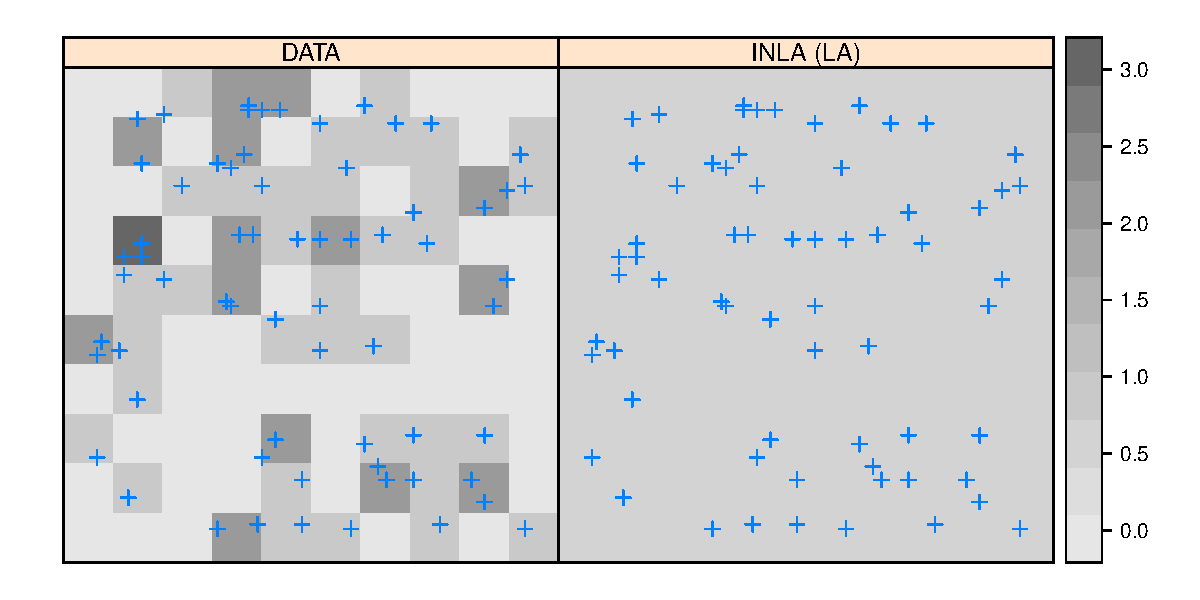
\includegraphics{spatial_inla-008}
\end{center}
\caption{Estimation of the intensity of a point pattern with \pkg{R-INLA}, 
Japanese black pine dataset.}
\label{fig:sppa}
\end{figure}



\subsection{Geostatistics}


\pkg{R-INLA} deals with geostatistical data on a regular grid. This means
that observations need to be matched to the points in the grid and that those
points with no observations attached are considered as missing values.
Hence, this is somewhat similar to the analysis of lattice data and point
patterns. However, \pkg{R-INLA} provides a number of options to build 
model-based geostatistical models \citet{DiggleRibeiro:2007} First
of all, different likelihoods can be used. Secondly, there are different
options to define the spatial random effects. Although it is still possible
to model spatial dependence in the grid of points using a CAR specification,
\pkg{R-INLA} provides a two-dimensional Mat\'ern covariance function. 


This correlation allows, for example, the use of exponentially decaying
functions suc as 

$$
\Sigma_{ij} = \sigma^2 \exp(-d_{ij}/\varphi)
$$
\noindent
where $d_{ij}$ is the distance between points $i$ and $j$, and $\varphi$
is a parameter that controls the scale of the spatial dependence.


%
%IMPORTANT: CHange the text if used in the paper
%
%In this acse, the variance-covariance matrix is defined as 
%
%$$
%\Sigma_{ij}= \sigma^2 \frac{\tau^{\kappa} K(\tau, \kappa)}{2^{\kappa-1} \Gamma(\kappa)}; \tau = \alpha_{\kappa}d_{ij}/\varphi
%$$
%\noindent
%$K(\cdot, \kappa)$ is the modified Bessel function of order $\kappa$ and
%$\Gamma(\cdot)$ the Gamma function. $\alpha_{\kappa}$ and $\varphi$ can be used
%to control the scale of the spatial variation. Setting $\kappa$ to $0.5$
%leads to an exponential covariance. Other values of $\kappa$ will lead
%to other known spatial covariance functions \citep{ISI:000263326600001}.



More rencetly, \citet{Lindgren:2011} follow a different approach based on
a triangulation on the sampling points and the use of stochastic partial
differential equations. Now, the spatial effects are defined as

$$
u(s)=\sum_{k=1}^n \psi_k(s)w_k,\ s\in \mathbb{R}^2
$$
\noindent
Here, $\{\psi_k(s)\}$ are a basis of functions and $w_k$ are associated
weights. Weights are assumed to be Gaussian. The advantages of this approach
for sptial statistics are is fully described in \citet{Camelettietal:2013}.


In order to show how to fit geostatistical models with \pkg{R-INLA} we
reproduce here an example from \citet{GomezRubioetal:2013} based on the
Rongelap data set \citep{DiggleRibeiro:2007}, which records  radionuclide
concentration at 157 different locations in Rongelap island. We have restricted
the analysis to one of the clusters in the north-east part of the island
because obervations need to be matched to a regular grid of points.

\begin{Schunk}
\begin{Sinput}
> library("geoR")
> library("geoRglm")
> data("rongelap")
> rgldata <- as.data.frame(rongelap)
> nrow = 5
> ncol = 5
> n = nrow * ncol
> xy <- rongelap[[1]]
> idx1 <- (xy[, 1] < -500 & xy[, 1] > -700 & xy[, 2] > -1900 & 
+     xy[, 2] < -1700)
> idx2 <- (xy[, 1] < -300 & xy[, 1] > -500 & xy[, 2] > -1500 & 
+     xy[, 2] < -1300)
> xxyy <- SpatialPoints(rbind(xy[idx1, ], xy[idx2, ]))
> rgldata <- rgldata[idx1, ]
\end{Sinput}
\end{Schunk}

\begin{Schunk}
\begin{Sinput}
> grd <- GridTopology(cellcentre.offset = c(min(rgldata$X1), min(rgldata$X2)), 
+     cellsize = c(diff(range(rgldata$X1))/(nrow - 1), diff(range(rgldata$X2))/(ncol - 
+         1)), cells.dim = c(nrow, ncol))
> inla2sp <- as.vector((inla.lattice2node.mapping(nrow, ncol))[, 
+     ncol:1])
> spgrd <- SpatialGridDataFrame(grd, as.data.frame(rgldata[inla2sp, 
+     ]))
> polygrd <- as(grd, "SpatialPolygons")
> dataidx <- overlay(SpatialPoints(as.matrix(rgldata[, 1:2])), 
+     polygrd)
> yag <- by(rgldata$data, dataidx, sum)
> umag <- by(rgldata$units.m, dataidx, sum)
> ratioag <- yag/umag
> spgrd$ratioag <- NA
> spgrd$ratioag[as.numeric(names(ratioag))] <- ratioag
> spgrd$SPIDX <- 1:nrow(spgrd)
> spgrd$INLAIDX <- inla2sp
> rongelap2 <- as.geodata(cbind(coordinates(spgrd)[!is.na(spgrd$ratioag), 
+     ], spgrd$ratioag[!is.na(spgrd$ratioag)]))
\end{Sinput}
\end{Schunk}


Here we define a model with an intercept term and a random effect of the
Mat\'ern class. Note how we have fixed, for convenience, 
the value of the range and precision.

\begin{Schunk}
\begin{Sinput}
> formula <- ratioag ~ 1 + f(spgrd$INLAIDX, model = "matern2d", 
+     nrow = nrow, ncol = ncol, hyper = list(range = list(initial = log(sqrt(8)/0.5), 
+         fixed = TRUE), prec = list(initial = log(1), fixed = TRUE)))
> rglinlala <- inla(formula, family = "poisson", control.predictor = list(compute = TRUE), 
+     control.compute = list(dic = TRUE), data = as.data.frame(spgrd))
> spgrd$INLALA <- rglinlala$summary.fitted.values[, 1]
\end{Sinput}
\end{Schunk}

Figure \ref{fig:geos} shows the observed and estimated radionuclide
concentration in Rongelap island. It can be seen how our model has spatially
smoothed the observed values.

\begin{figure}[h]
\begin{center}
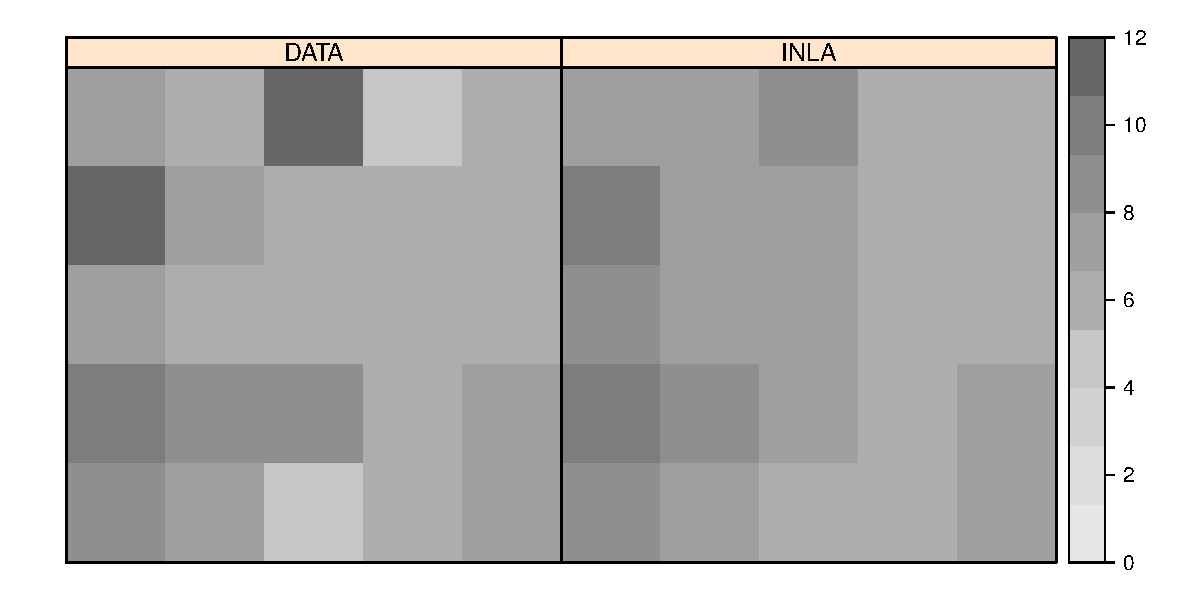
\includegraphics{spatial_inla-012}
\caption{Observed (left) and estimated (right) of radionuclide concentration
in Rongelap island.}
\label{fig:geos}
\end{center}
\end{figure}



\section[Extending {R-INLA} to fit new models]{Extending \pkg{R-INLA} to fit new models} 

\label{sec:extINLA}


Although the current implementation of INLA in the \pkg{R-INLA} package
provides a reasonable number of models for spatial dependence it may be the
case that we need to include some other models. As it is now, this is not
possible.

\citet{Bivandetal:2013} describe a simple way of extending INLA to use other
latent models.  In particular they focus on some latent models used in spatial
econometrics and which are not available as part of the \pkg{R-INLA} package at
the moment.

This approach is based on considering a model where one or several have been
fixed in a way that makes the conditioned model fitable with \pkg{R-INLA}.  If
we denote by $\rho$ the vector of parameters to fix and by $\hat{\rho}$ the
fixed parameters,  the full posterior marginal could be written as


$$
\pi(\mathbf{x}, \mathbf{\theta}|\mathbf{y}, \hat{\rho}) 
$$
\noindent
Taking this into account,  it is clear that when conditioning on
$\rho=\hat\rho$ \pkg{R-INLA} will give us an approximation to
$\pi(x_i|\mathbf{y}, \hat{\rho})$ and $\pi(\theta_i|\mathbf{y}, \hat{\rho})$.



Note that the full posterior distribution can be obtained by integrating $\rho$,
i.e.,

\begin{equation}
\pi(\mathbf{x}, \mathbf{\theta}|\mathbf{y}) = 
\int \pi(\mathbf{x}, \mathbf{\theta}|\mathbf{y}, \rho)\pi(\rho|\mathbf{y})d\rho
\label{eq:fullpost}
\end{equation}
\noindent
where $\pi(\rho|\mathbf{y})$ is the posterior distribution of $\rho$. Also,
note that this can be written as

\begin{equation}
\pi(\rho|\mathbf{y}) \propto \pi(\mathbf{y}|\rho) \pi(\rho)
\label{eq:postrho}
\end{equation}
\noindent
Here $\pi(\rho)$ is a prior distribution on $\rho$ and $\pi(\mathbf{y}|\rho)$
is the marginal likelihood of the model, which is reported by \pkg{R-INLA}.
Hence, $\pi(\rho|\mathbf{y})$ can be estimated by re-scaling expression 
(\ref{eq:postrho}).


The posterior distribution of $\rho$ can be estimated by defining a fine grid
of values so that $S=\{\rho_i\}_{i=1}^r$ and $\pi(\rho_i|\mathbf{y})$ is
computed.  Then $\pi(\rho|\mathbf{y})$ can be obtained by fitting and
re-scaling a spline (or other non-linear function) to the previous values.
Using simple numerical integration techniques we can obtain an approximation to
$\pi(\mathbf{x}, \mathbf{\theta}|\mathbf{y})$ as follows:

\begin{equation}
\pi(\mathbf{x}, \mathbf{\theta}|\mathbf{y}) = \int \pi(\mathbf{x}, \mathbf{\theta}|\mathbf{y}, \rho)\pi(\rho|\mathbf{y})d\rho
\simeq
\sum_{\rho_i\in S}\pi(\mathbf{x}, \mathbf{\theta}|\mathbf{y}, \rho_i)  
\pi(\rho_i|\mathbf{y}) \Delta_i
\label{eq:fullpostapp}
\end{equation}
\noindent
where $\Delta_i$ is the amplitude of the interval used in the discretization
of $\rho$.

Note that the previous expression can be regarded as a weighted average
of the different models fitted after conditioning on different values of
$\rho$.

From equation \ref{eq:fullpostapp} it is clear that we can obtain the following
approximations to the posterior marginals of the individual latent parameters
and hyperparameters:

$$
\hat{\pi}(x_i|\mathbf{y}) = \sum_i \pi(x_i|\mathbf{y}, \rho_i) w_i
$$

$$
\hat{\pi}(\theta_i|\mathbf{y}) = \sum_i \pi(\theta_i|\mathbf{y}, \rho_i) w_i
$$
\noindent
$w_i$ is a weight associated with $\rho_i$ as follows:

$$
w_i = \pi(\rho_i|\mathbf{y})\Delta_i
$$

This is like making a Bayesian Model Averaging \citep{Hoetingetal:1999} on the
different conditioned models fitted with \pkg{R-INLA}. Altogether, this
provides a way of combining simpler models to obtain our desired model. In
Section \ref{sec:examples} we show how to apply these ideas to different models
in spatial and spatio-temporal statistics.


%If $\rho$ is a discrete parameter with values in a (finite) set $S$, this can 
%be done by
%
%$$
%\pi(\rho|\mathbf{y}) = \frac{\pi(\mathbf{y}|\rho) \pi(\rho)}{\sum_{\rho_i\in S} \pi(\mathbf{y}|\rho_i) \pi(\rho_i) }
%$$

Note that this approach can be easily extended to the case of $\rho$ being
a discrete random variable.


\subsection{Implementation}

We have implemented this approach in an \pkg{R} package called \pkg{INLABMA},
available from \url{http://r-forge.r-project.org}. The package includes some
general functions to conduct Bayesian Model Averaging of models fitted with
INLA. In addition, we have included some wrapper functions to fit the models
described in Section \ref{sec:examples}.


\section{Examples}
\label{sec:examples}

\subsection{Leroux model}

\citet{Lerouxetal:1999} propose a model for the analysis of spatial data in a
lattice which is similar to the one by \citet{besagetal:1991}, in the sense
that they split variation according to  spatial and non-spatial patterns.
Rather than including the spatial and non-spatial random effect as a sum in the
linear term they consider a single random effects as follows:

\begin{equation}
u \sim MVN(0, \Sigma);\ \Sigma=\sigma^2 ((1-\lambda) I_n+\lambda M)^{-1}
\label{eq:leroux}
\end{equation}
\noindent
Here $M$ is the precision matrix of a process with spatial structure and we
will take that of an instrinsic CAR specification. Hence, the precision matrix
is, in a sense, a mixture of the precisions of a non-spatial and a spatial
one. $\lambda$ controls how strong the spatial structure is. For $\lambda=1$
the effect is entirely spatial whilst for $\lambda=0$ there is no spatial
dependence.

In principle, this is not a model that \pkg{R-INLA} can fit. However, if
$\lambda$ is fixed, then the random effects are Gaussian with a known structure
for the variance-covariance matrix which can be fitted using a \code{generic0}
latent model.

\subsubsection{Boston housing data}

Here we revisit the Boston housing data to fit the Leroux et al. model.  First
of all, it is worth mentioning that the model needs a wrapper function to be
fitted for a given value of the spatial parameter $\lambda$. This
wrapper function is included in the \proglang{R} package \pkg{R-INLA}.

It is based on the \code{generic0} latent model available in  \pkg{R-INLA}.
This model implements a multivariage Gaussian random effect with zero mean and
precision matrix as in equation (\ref{eq:leroux}). Once $\lambda$ is fixed the
model can be easily fitted with \pkg{R-INLA}.  We repeat this procedure for
different values of $\lambda$ to obtain a list of fitted models to be combined
later.

Hence, we can write a similar wrapper function as in the previous example for
the spatial econometrics models, which is included in package \pkg{INLABMA}:

\begin{Schunk}
\begin{Sinput}
> library("INLABMA")
> leroux.inla
\end{Sinput}
\begin{Soutput}
function (formula, d, W, lambda, improve = TRUE, fhyper = NULL, 
    ...) 
{
    W2 <- diag(apply(W, 1, sum)) - W
    Q <- (1 - lambda) * diag(nrow(W)) + lambda * W2
    environment(formula) <- environment()
    if (is.null(fhyper)) {
        formula <- update(formula, . ~ . + f(idx, model = "generic0", 
            Cmatrix = Q))
    }
    else {
        formula <- update(formula, . ~ . + f(idx, model = "generic0", 
            Cmatrix = Q, hyper = fhyper))
    }
    res <- inla(formula, data = d, ...)
    if (improve) 
        res <- inla.hyperpar(res, diff.logdens = 20)
    res$logdet <- as.numeric(determinant(Q)$modulus)
    res$mlik <- res$mlik + res$logdet/2
    return(res)
}
<environment: namespace:INLABMA>
\end{Soutput}
\end{Schunk}


In the previous code, the precision matrix is created using the adjacency
matrix and the value of $\lambda$. Then the \code{generic0} model is added to the
formula with the fixed effects. Finally we correct the marginal log-likelihood
$\pi(\mathbf{y})$ by adding the log-determinat of $(1-\lambda)I_n+\lambda M)$.
Note that, in principle, this is not needed to fit a single model and obtain
the approximations to the posterior marginals as it is a constant. However, we
are fitting and combining several models so we need to correct for this
becuase this scaling factor will change with the value of $\lambda$.
Argument \code{'...'} is used to pass any other options to \code{inla()}. 
This can be used to tune and set a number of other options.

Similar wrapper functions can be written for other models. The functions
included in package \pkg{INLABMA} are similar, but include further options
\citep[see,][for details]{Bivandetal:2013}.

%Note that here \code{zero.variance} is used to set
%to zero the additional error term which is added by default by \pkg{R-INLA}.


Also, the adjacency matrix is taken from the data provided in the \code{boston}
data set.
Note that we will be using a binary adjacency matrix as the random
effects have an intrinsic CAR specification:
\begin{Schunk}
\begin{Sinput}
> #Binary adjacency matrix
> boston.matB<-listw2mat(nb2listw(boston.soi, style="B"))
> bmspB<-as(boston.matB, "CsparseMatrix")
\end{Sinput}
\end{Schunk}

Function \code{inla.leroux} is used in the example below to compute the fitted
models for the Leroux et al. model.  In this case, we take $\lambda$ to be in
the interval $(0.8,0.99)$ after previous assessment on where
$\pi(\lambda|\mathbf{y})$ has its mode. Also, we define a prior for the
precission of the random effects in variable \code{fhyper}.

\begin{Schunk}
\begin{Sinput}
> #Run models
> rlambda<-seq(0.8, .99, length.out=15)
> #Setting of hyper-parameters
> fhyper=list(prec=list(prior="loggamma", param=c(1,1), initial=log(1), fixed=FALSE))
> #Formula
> form2<-log(CMEDV) ~ CRIM + ZN + INDUS + CHAS + I(NOX^2) + I(RM^2) + 
+     AGE + log(DIS) + log(RAD) + TAX + PTRATIO + B + log(LSTAT)
\end{Sinput}
\end{Schunk}

\begin{Schunk}
\begin{Sinput}
> lerouxmodels = mclapply(rlambda,
+         function(lambda) {
+                 leroux.inla(form2, d=boston.c, W=boston.matB, lambda=lambda,
+                         fhyper=fhyper, improve=TRUE,
+                         family = "gaussian",
+ #   control.family = list(hyper = zero.variance),
+                         control.predictor=list(compute=TRUE),
+                         control.compute=list(dic=TRUE, cpo=TRUE),
+                         control.inla=list(print.joint.hyper=TRUE), verbose=FALSE
+                 )
+         })
\end{Sinput}
\end{Schunk}






Following this, we need to combine the different models to obtain the final
model by Bayesian Model Averaging. We will take a uniform prior on $\rho$ and
set the third argument in the following function to $1$. Note that another
prior can be used here by giving the density of the prior at the different
values of $\rho$.



\begin{Schunk}
\begin{Sinput}
> bmaleroux<-BMA2(lerouxmodels, rlambda, 0, impacts=FALSE)
\end{Sinput}
\end{Schunk}


\noindent
\code{bmaleroux} is similar to the object returned by \code{inla()} and it
includes the posterior marginals and summary statistics for $\lambda$
in a list element named \code{rho}. This provides summary statistics (mean,
standard deviation, some quantiles and the posterior marginal.

The same model can be fitted usig package \pkg{CARBayes}\citep{CARBayes:2013}
as follows:

\begin{Schunk}
\begin{Sinput}
> #Run with CARBAYES
> library("CARBayes")
> 
> #New model
> #form2<-log(CMEDV) ~CRIM+ZN + INDUS + CHAS + I(NOX^2)+
> #   I(RM^2) +  AGE + log(DIS) + log(RAD) + TAX + PTRATIO + B + log(LSTAT)
> 
\end{Sinput}
\end{Schunk}
\begin{Schunk}
\begin{Sinput}
> attach(boston.c)
> lcarbayes<- gaussian.lerouxCAR (form2, W=as.matrix(bmspB), burnin=500, 
+    n.sample=2500, thin=5)
> detach(boston.c)
\end{Sinput}
\end{Schunk}


Table \ref{tab:leroux} shows point estimates and standard deviations of the
fixed effects and parameter $\lambda$ (bottom line) in the model. It is clear
that there are no significant differences between the estimates computed with
MCMC and our method.  Furthermore, Figure \ref{fig:leroux} shows the marginal
distribution of $\lambda$ and it shows how our estimate is very close to that
provided by MCMC. The slight difference that is observed may well be due to the
fact that different priors have been used for the variances of the random
effects and the error term. \pkg{CARBayes} uses uniform priors on the variances,
whiles \pkg{R-INLA} assigns inverted Gamma distributions to the variances.

% latex table generated in R 3.0.1 by xtable 1.7-1 package
% Fri May 31 13:35:40 2013
\begin{table}[ht]
\centering
\begin{tabular}{rrrrr}
  \hline
 & Mean (INLA) & SD (INLA) & Mean (MCMC) & SD (MCMC) \\ 
  \hline
(Intercept) & 3.5257 & 0.1691 & 3.5514 & 0.1790 \\ 
  CRIM & -0.0048 & 0.0009 & -0.0051 & 0.0010 \\ 
  ZN & 0.0004 & 0.0005 & 0.0004 & 0.0005 \\ 
  INDUS & -0.0003 & 0.0026 & -0.0002 & 0.0027 \\ 
  CHAS1 & -0.0258 & 0.0285 & -0.0225 & 0.0292 \\ 
  I(NOX\verb|^|2) & -0.1206 & 0.1566 & -0.0850 & 0.1683 \\ 
  I(RM\verb|^|2) & 0.0110 & 0.0011 & 0.0108 & 0.0011 \\ 
  AGE & -0.0013 & 0.0005 & -0.0012 & 0.0005 \\ 
  log(DIS) & -0.0906 & 0.0622 & -0.0959 & 0.0634 \\ 
  log(RAD) & 0.0516 & 0.0210 & 0.0549 & 0.0225 \\ 
  TAX & -0.0004 & 0.0001 & -0.0004 & 0.0001 \\ 
  PTRATIO & -0.0173 & 0.0053 & -0.0184 & 0.0057 \\ 
  B & 0.0007 & 0.0001 & 0.0007 & 0.0001 \\ 
  log(LSTAT) & -0.2262 & 0.0222 & -0.2295 & 0.0246 \\ 
  lambda & 0.9493 & 0.0294 & 0.9537 & 0.0262 \\ 
   \hline
\end{tabular}
\caption{Point estimates of fixed effects using INLA and MCMC.} 
\label{tab:leroux}
\end{table}

\begin{figure}[h]
\begin{center}
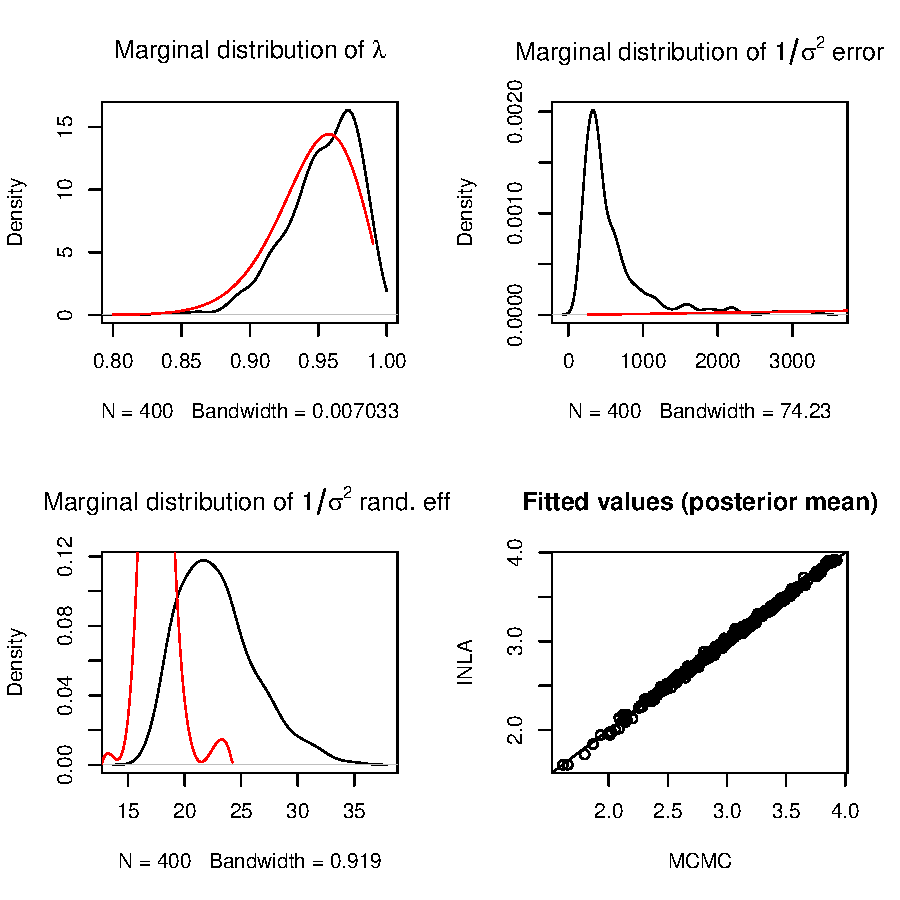
\includegraphics{spatial_inla-027}
\end{center}
\caption{Comparisson between the posterior marginals of several parameters in 
Leroux et al.'s model and fitted values with INLA and MCMC.}
\label{fig:leroux}
\end{figure}

While writting this paper, \citet{LeeMitchell:2013} have come up with an
alternative way of fitting this model using \pkg{R-INLA} and a \code{generic1}
latent model. In general, the results obtained with our approach are very
similar to the ones obtained with theirs for the Boston housing data.








\subsection{Spatial econometrics models}

\citet{LeSagePace:2009} describe a good deal of models amply used in spatial
econometrics. These models have been developed to make it explicit that there
is dependence among the observed values $y_i$. First of all, spatial dependence
can be assumed on the error term, so that we have a slightly different model:

\begin{equation}
y= \alpha+\beta X +u; u=\rho W u+\varepsilon
\end{equation}
\noindent
Here the error term $u$ is assumed to have spatial dependence.  $\rho$ is a
parameter that controls spatial autocorrelation, $\alpha$ is the intercept, $X$
a design matrix of covariates and $\beta$ a vector of associated coefficients.
$\varepsilon$ is an error term which is Gaussian with zero mean and
variance-covariance matrix $\Sigma$. Here, $\Sigma = \sigma^2 I_n$ with $I_n$
being a $n\times n$ identity matrix and $\sigma^2$ is the variance of the error
term.


The adjacency matrix $W$ is often taken to be row-standadrised \citep[see, for
example,][]{Haining:2003} to ensure that $\rho$ in the interval $(-1, 1)$.
Also, when $\rho$ is equal to zero there is no spatial dependence.

This can be reformulated as

\begin{equation}
y= \alpha+\beta X+\varepsilon'
\end{equation}
\noindent
$\varepsilon '$ is now an error term with a Gaussian distribution with zero
mean and variance-covariance matrix $\Sigma=((I_n-\rho W)(I_n-\rho W'))^{-1}$.
Note that this variance-covariance encodes spatial dependance in a particular
way and that this is often referred to as Spatial Autoregressive (SAR)
specification.


Alternatively, autocorrelation can be modelled explicitely so that the
variable response $y$ depends on itself as follows:

$$
y= \alpha+\beta X+\rho W y +\varepsilon 
$$
\noindent
This model can be reformulated as

\begin{equation}
y = (I_n-\rho W)^{-1}(\alpha+\beta X)+\varepsilon ' 
\label{eq:slm}
\end{equation}
\noindent
where $\varepsilon '$ is a Gaussian term with zero mean and
variance-covariance matrix with a SAR specification.

In addition to the previous models, sometimes lagged covariates are 
added to include the effects of neighbouring covariates. This is known
as Spatial Durbin Model  and it is often expresed as

$$
y= \rho W y+ \alpha+\beta X+\gamma W X +\varepsilon 
$$
\noindent
which leads to

$$
y= (I_n-\rho W)^{-1}(\alpha+\beta X+\gamma W X) +\varepsilon '
$$
\noindent
Note that this is like our previopus model \ref{eq:slm} using an extended desgn
matrix that includes both $X$ and $W X$.

These models cannot be fitted with \pkg{R-INLA} for two reasons. First of all, 
the SAR specification is not implemented, so we cannot consider it for out
error terms. Furthermore, it is not posible to define a model 
where the linear predictor is multiplied by $(I_n-\rho W)^{-1}$.

Following Section \ref{sec:extINLA}, it should be noted that, for a fixed
$\rho$ these models become standard linear models with a particular 
(but known) design matrix for the fixed effects and a multivariate Gaussian
distribution with zero mean and variance-covariance matrix.

This model can be easily fitted using \pkg{R-INLA} for different values
of $\rho$. Note that, according to \citet{Haining:2003}, $\rho$ is constrained 
to be in the interval $(1/\lambda_{min}, 1/\lambda_{max})$, with
$\lambda_{min}$ and $\lambda_{max}$ the minimum and maximum eigenvalues of
the adjacency matrix $W$. For row standardised adjacency matrices we have that
$\lambda_{max}=1$ and then $\rho$ is lower than 1. Furthermore, we are often
interested in positive spatial autocorrelation and, in practice, we will
assume that $\rho$ is in the interval $[0,1)$.


Finally, we have considered here the Gaussian case, but it is very easy to
extend this model to consider other likelihoods. In particular,
\citet{LeSageetal:2011} describe a Spatial Probit model where the outcome is
whether an event occured. Hence, the response and the linear predictors are
linked via a probit function as follows:

$$
y_i=
\left\{
\begin{array}{cc}
1 & if y^*_i\geq 0\\
0 & if y^*_i < 0
\end{array}
\right.
$$

The previous approach can be used here as well. The same code will still work
as we can define a different family and link function to be used when calling
\code{inla()}.

\subsubsection{Boston housing data}

Here we revisit the Boston housing data to fit the three models on Spatial
Econometrics described here. First of all, it is worth mentioning that each
models needs a wrapper function to be fitted for a given value of the
spatial autocorrelation parameter $\rho$. These wrapper functions are
included in \proglang{R} package \pkg{R-INLA}.

All functions are based on the \code{generic0} model available in  \pkg{R-INLA}.
This model implements a multivariage Gaussian random effect with zero mean
and precision matrix $\frac{1}{\sigma^2} Q$. Once $\rho$ is fixed, $Q$ is
known and the model can be easily fitted with \pkg{R-INLA} for that value of
$\rho$. We repeat this procedure for different values of $\rho$ to
obtain a list of fitted models to be combined later.

\begin{Schunk}
\begin{Sinput}
> library("INLABMA")
\end{Sinput}
\end{Schunk}

A simple wrapper function can be defined as follows for the SEM model:

\begin{Schunk}
\begin{Sinput}
> semwr.inla<-function(formula, d, W, rho,...)
+ {
+         IrhoW<-diag(nrow(W))-rho*W
+         IrhoW2<-IrhoW%*%t(IrhoW)
+ 
+         environment(formula)<-environment()
+ 
+         formula<-update(formula,
+           . ~ . + f(idx, model="generic0", Cmatrix =IrhoW2) )
+ 
+         res<-inla(formula, data=d, ...)
+ 
+   #Compute log-determinat to correct the marginal-loglikelihood
+         res$logdet<-as.numeric(determinant(IrhoW2)$modulus)
+         res$mlik<-res$mlik+res$logdet/2
+ 
+         return(res)
+ }
\end{Sinput}
\end{Schunk}

In the previous code, the precision matrix is created using the adjacency
matrix and the value of $\rho$. Then the \code{generic0} model is added to the
formula with the fixed effects. Finally we correct the marginal log-likelihood
$\pi(\mathbf{y})$ by adding the log-determinat of $(I_n-\rho W')(I_n-\rho W)$.
Note that, in principle, this is not needed to fit a single model and obtain
the approximations to the posterior marginals as it is a constant. However, we
are fitting and combining several models so we need to correct for this
becuase this scaling factor will change with the value of $\rho$.
Argument \code{'...'} is used to pass any other options to \code{inla()}. 
This can be used to tune and set a number of other options.

Similar wrapper functions can be written for the other models. The functions
included in pakcage \pkg{INLABMA} are similar, but include further options,
to improve fitting or compute the impacts 
\citep[see,][for details]{Bivandetal:2013}.

This is used in the following example to compute the fitted models
for the SEM model. Note that here \code{zero.variance} is used to set
to zero the additional error term which is added by default by \pkg{R-INLA}.
Also, the adjacency matrix is taken from the data provided in the \code{boston}
data set.

\begin{Schunk}
\begin{Sinput}
> zero.variance = list(prec = list(initial = 25, fixed = TRUE))
> boston.mat <- nb2mat(boston.soi)
> bmsp <- as(boston.mat, "CsparseMatrix")
> boston.c$idx <- 1:nrow(boston.c)
\end{Sinput}
\end{Schunk}

Next, we define a fine grid on the interval $(0,1)$ to give values
to $\rho$ and compute the different models under these values. Here
we have used \code{mclapply} to parallelise the computations. Note
that this is an advantage of fitting this conditioned models compared 
standard MCMC methods.


\begin{Schunk}
\begin{Sinput}
> fform<-log(CMEDV) ~CRIM+ZN + INDUS + CHAS + I(NOX^2)+
+    I(RM^2) +  AGE + log(DIS) + log(RAD) + TAX + PTRATIO + B + log(LSTAT)
> rrho1<-seq(0.5, .9, len=20)
\end{Sinput}
\end{Schunk}
\begin{Schunk}
\begin{Sinput}
> semmodels = mclapply(rrho1,
+         function(rho) {
+                 sem.inla(fform, d=boston.c, W=boston.mat, rho=rho,
+                         family = "gaussian", impacts=FALSE,
+                         control.family = list(hyper = zero.variance),
+                         control.predictor=list(compute=TRUE),
+                         control.compute=list(dic=TRUE, cpo=TRUE),
+                         control.inla=list(print.joint.hyper=TRUE), verbose=FALSE
+                 )
+         })
\end{Sinput}
\end{Schunk}

\noindent
Following this, we need to combine the different models
to obtain the final model by Bayesian Model Averaging. We will take
a uniform prior on $\rho$ and set the third argument in the following
function to $1$. Note that another prior can be used here by giving
the density of the prior at the different values of $\rho$.

\begin{Schunk}
\begin{Sinput}
> bmasem<-BMA2(semmodels, rrho1, 1 , impacts=FALSE)
\end{Sinput}
\end{Schunk}

\code{bmasem} is similar to the object returned by \code{inla()} and it
includes the posterior marginals and summary statistics for $\rho$.


SLM and SDM models can be fitted using similar code. In the case of
the SLM, first we compute the design matrix (of the fixed effects) 
to be used later when fitting the models. This will speed up the 
computations.

\begin{Schunk}
\begin{Sinput}
> mmatrix<-model.matrix(fform, boston.c)
> rrho2<-seq(0.3, .6, len=20)
\end{Sinput}
\end{Schunk}

\begin{Schunk}
\begin{Sinput}
> slmmodels = mclapply(rrho2,
+         function(rho) {
+                 slm.inla(form, d=boston.c, W=boston.mat, rho=rho, mmatrix=mmatrix,
+                         family = "gaussian", impacts=TRUE,
+                         control.data = list(hyper = zero.variance),
+                         control.predictor=list(compute=TRUE),
+                         control.compute=list(dic=TRUE, cpo=TRUE),
+                         control.inla=list(print.joint.hyper=TRUE), verbose=FALSE
+                 )
+         })
> 
\end{Sinput}
\end{Schunk}

\begin{Schunk}
\begin{Sinput}
> bmaslm<-BMA2(slmmodels, rrho2, 1 , impacts=FALSE)
\end{Sinput}
\end{Schunk}

In the case of the SDM, it is very helpful to compute $X$ and $WX$ beforehand
to reduce computation time, as this is common to all the fitted models
regarless of the value of $\rho$. This can be later passed to wrapper function
\code{sdm.inla}.

\begin{Schunk}
\begin{Sinput}
> mmW<-bmsp%*%mmatrix[,-1]#Remove intercept
> mmatrixsdm<-cbind(mmatrix, as.matrix(mmW))
> rrho3<-seq(0.4, .7, len=20)
\end{Sinput}
\end{Schunk}

\begin{Schunk}
\begin{Sinput}
> sdmmodels = mclapply(rrho3,
+         function(rho) {
+                 sdm.inla(form, d=boston.c, W=boston.mat, rho=rho, mmatrix=mmatrixsdm,
+                         family = "gaussian", impacts=TRUE,
+                         control.data = list(hyper = zero.variance),
+                         control.predictor=list(compute=TRUE),
+                         control.compute=list(dic=TRUE, cpo=TRUE),
+                         control.inla=list(print.joint.hyper=TRUE), verbose=FALSE
+                 )
+         })
\end{Sinput}
\end{Schunk}

\begin{Schunk}
\begin{Sinput}
> bmasdm<-BMA2(sdmmodels, rrho3, 1 , impacts=FALSE)
\end{Sinput}
\end{Schunk}

As we have seen in the previous examples, combining the different values 
for the different values of $\rho$ provides accurate estimates of the posterior
marginals for the model parameters. The estimates of the marginals of
$\rho$ can be found in Figure \ref{fig:pmargrho}.

\begin{figure}[h]
\begin{center}
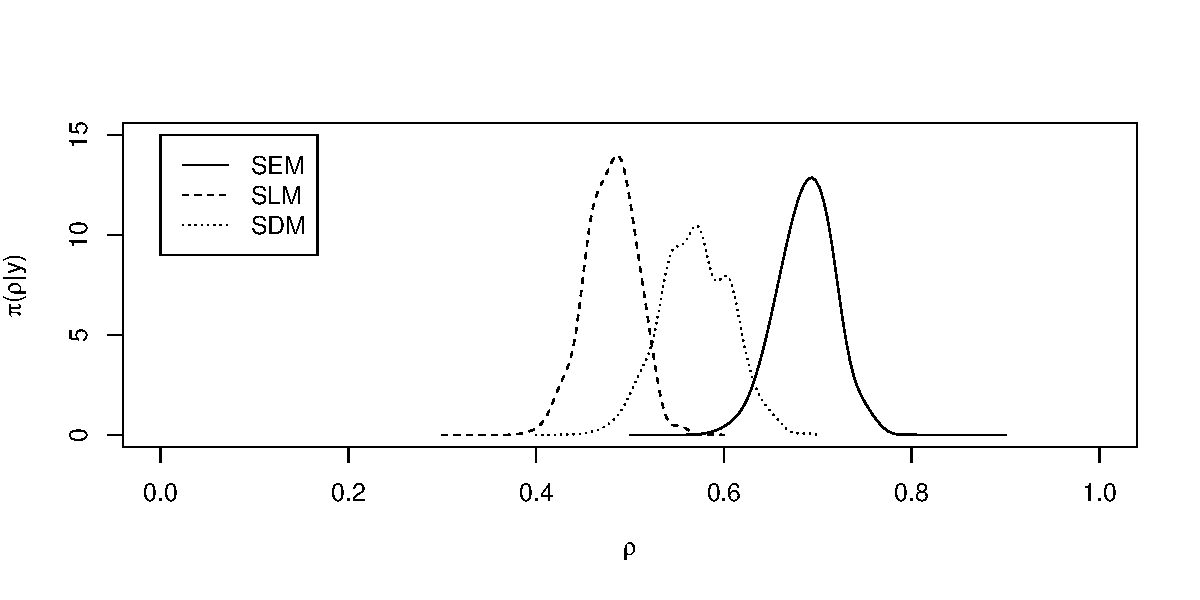
\includegraphics{spatial_inla-044}
\end{center}
\caption{Posterior marginal of the spatial autocorrelation parameter $\rho$
for different spatial models.}
\label{fig:pmargrho}
\end{figure} 



%\subsection{Model Selection with INLA and RJMCMC}

%\subsubsection{Boston Housing Data}

%\subsection{Spatio-temporal models}
%
%Spatio-temporal models can be easily fitted with \pkg{R-INLA} when the spatial
%and temporal effects are separable. However, it may be a complex issue when 
%
%\subsubsection{Cancer in New Mexico}



\section{Discussion} \label{sec:disc}

The Integrated Nested Laplace Approximation has provided a new paradigm to
model fitting in Bayesian analysis. By focusing on the marginals and providing
an interesting computational approach, it has provided an reasonable and faster
alternative to MCMC. Furthermore, the \pkg{R-INLA} package makes model fitting
in \pkg{R} a very simple task.  Although \pkg{R-INLA} implements some key
models, there are some others that have not been implemented yet.
In addition, it is not easy to implement completely new models within the
\pkg{R-INLA}.

In this paper we have shown an innovative approach to model fitting with INLA
and \pkg{R-INLA} which increases the number of latent models that can be fitted
with INLA. We have been able to do so by fitting conditional models on some
model parameters and combining the resulting models using simple methods for
Bayesian model averaging. We have considered the case in which conditioning is
carried out on a single parameter but our approach can be easily extended to the
case of more than one parameter.

Given that the different models can be run in parallel, this is not a real
computational burden. In our examples, 20 models seemed to be enough to obtain
good approximations. Implementing new models is very simple and the wrapper
functions included in the examples and the \pkg{INLABMA} package provide
templates to start with.

Other computationally efficient approaches for Bayesian inference on spatial 
models include, for example, \pkg{RStan} \citep{stan-software:2013}.
It provides an efficient MCMC algorithm and provides a good number of options
for Gaussian processes which can be used to implement some of the models
described in this paper. It is worth mentioning that \pkg{RStan} models are not
based on \pkg{R} code but on \pkg{C++} code that is compiled once the main
model is defined.

We have shown that this is a practical approach using different examples in
spatial statistics. Similarly, complex spatio-temporal models could be fitted
using a similar approach. However, it should be noted that our approach can be
extended to other areas.

\section{Acknowledgements}

We would like to thank Duncan Lee and Lola Ugarte for their help and comments
on how to fit the Leroux model with \pkg{R-INLA}.


%\bibliography{INLA_econometrics,RS_handbook_SpatStat_INLA,JSSpaper}
\bibliography{biblio.bib}


\end{document}
